\chapter{Entanglement Generation With a Quantum Networking Stack}
\label{chp:netstack}

\begin{abstract}
Entanglement generation has already been demonstrated a few times today, at various node-to-node
distances, on several quantum physical platforms, and mostly on small-scale quantum networks.
Scaling current quantum communication demonstrations to a large-scale quantum network will require
not only advancements in quantum hardware capabilities, but also robust control of such devices to
bridge the gap in user demand. Moreover, the abstraction of tasks and services offered by the
quantum network should enable platform-independent applications to be executed without the knowledge
of the underlying physical implementation. In this chapter, we experimentally demonstrate
entanglement generation through \acrshort{qnodeos} and its quantum networking stack.
The link layer abstracts the physical-layer entanglement attempts into a robust,
platform-independent entanglement delivery service. The system is used to run full state
tomography of the delivered entangled states, as well as preparation of a remote qubit state on
a server by its client. Our results mark a clear transition from physics experiments to quantum
communication systems, which will enable the development and testing of components of future
quantum networks.
\end{abstract}

\note{This chapter is extracted from the npj paper. No major additions.}

\blfootnote{
    This chapter is based on the paper \citetitle{pompili_2022_experimental} by
    \textcite{pompili_2022_experimental}.
}

\newpage

\lettrine{N}{ear-term} quantum networks have already yielded successful experimental results towards
a future quantum internet. Fundamental primitives for entanglement-based quantum networks have been
demonstrated across several physical platforms, including trapped
ions~\cite{moehring_2007_ion_traps, stephenson_2020_highrate}, neutral
atoms~\cite{ritter_2012_elementary, hofmann_2012_heralded}, diamond color
centers~\cite{bernien_2013_heralded, kalb_2017_entanglement, humphreys_2018_delivery,
pompili_2021_multinode}, and quantum dots~\cite{delteil_2016_generation, stockill_2017_phasetuned}.
To scale up such physics experiments to intermediate-scale quantum networks, researchers have been
investigating how to enclose the complex nature of quantum entanglement generation into more robust
abstractions~\cite{aparicio_2011_protocol, dahlberg_2019_egp, pirker_2019_quantum,
kozlowski_2020_qnp, aguado_2020_enabling, kozlowski_2020_p4, alshowkan_2021_reconfigurable}.

A common way to facilitate the scalability of complex systems is to break down their architecture
into a stack of layers. Each layer in such a stack is characterized by a specific service that it
provides to the high layers, reducing complexity for the higher layers, which can subsequently rely
on this service. Moreover, the higher layers need no knowledge of the specific protocol and physical
realization that a lower layer uses to realize the specified service. An example from classical
networking is the \acrshort{tcpip} stack used on the present day internet. In this stack, the link
layer enables reliable transmission of data between two network nodes that are directly connected by
an unreliable physical medium such as fiber or radio. Higher layers can rely on errors being
detected by the link layer, and are agnostic about whether the underlying link layer protocol is
Ethernet or Wi-Fi.

Several network stacks have been proposed for quantum network nodes~\cite{dahlberg_2019_egp,
pirker_2019_quantum, kozlowski_2020_qnp}, like the one depicted in \cref{fig:netstack}. These draw
inspiration from classical architectures like the \acrshort{tcpip} stack or the more generic
\acrfull{osi} model. Specifically, the functional allocation of the stack proposed in
Ref.~\cite{dahlberg_2019_egp} conceptually mirrors the \acrshort{tcpip} stack in that the link layer
ensures reliable (quantum) communication between adjacent nodes, and the network layer extends this
service to nodes not directly connected by a physical medium themselves. We emphasize that of course
no quantum data is passed up and down the layers of the stack, but only qubit metadata. Very
intuitively, such metadata is similar to passing only references to an address in a physical memory
up and down the stack (similar to what happens in many implementations of the \acrshort{tcpip} stack
in practice), while in the classical case data may of course also be copied up and down layers.

We also note that the quantum internet, and the associated quantum network stack, do not aim to
replace the classical internet --- they will likely coexist, as the quantum internet cannot operate
without classical communication in practice. In addition to classical information used to facilitate
entanglement generation, we also expect classical communication at the level of the quantum
application itself (e.g.~quantum key distribution), which would for practical reasons be performed
using the classical internet. Finally, in a quantum network, classical communication could also be
used to realize controllers like those at the core of \acrfull{sdn}~\cite{ferguson_2021_orion} to
distribute information for resource scheduling and quality of service~\cite{skrzypczyk_2021_arch}.
The proposed quantum network stack architecture, along with proposals for resource scheduling and
routing techniques (e.g.~\cite{van_meter_2013_path, caleffi_2017_optimal,
gyongyosi_2018_decentralized, pant_2019_routing, chakraborty_2019_distributed, shi_2020_concurrent,
chakraborty_2020_entanglement, skrzypczyk_2021_arch}), pave the way for larger-scale quantum
networks.

In this work we experimentally demonstrate a link layer protocol for entanglement-based quantum
networks. The link layer abstracts the generation of entangled states between two physically
separated solid-state qubits into a robust and platform-independent service. An application can
request entangled states from the link layer and then, in addition, apply local quantum operations
on the entangled qubits in real-time. Using the link layer, we perform full state tomography of the
generated states and achieve remote state preparation --- a building block for blind quantum
computation --- as well as measuring the latency of the entanglement generation service.

To evaluate correct operation and performance of our system, we measure
\begin{inlinelist}
    \item the fidelity of the generated states and
    \item the latency incurred by link layer and physical layer when generating entangled pairs.
\end{inlinelist}
For both fidelity and latency, we find that our system performs with marginal overhead with respect
to previous non-platform-independent experiments. We also identify the sources of the additional
overhead incurred, and propose improvements for future realizations.

\begin{figure}
    \centering
    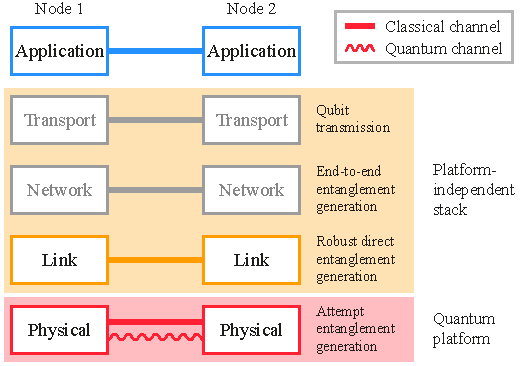
\includegraphics[width=0.6\linewidth]{figures/netstack.pdf}
    \caption{
        Quantum network stack architecture. At the bottom of the stack, the physical layer (red),
        which is highly quantum platform-dependent, is tasked with attempting entanglement
        generation. The link layer (yellow) uses the functionality provided by the physical layer to
        provide a platform-independent and robust entanglement generation service between
        neighboring nodes to the higher layers. Network and transport layer (not implemented in this
        work, grayed out) will support end-to-end connectivity and qubit transmission. Applications
        (blue) use the services offered by the stack to perform quantum networking tasks. Based on
        Ref.~\cite{dahlberg_2019_egp}.
    }
    \label{fig:netstack}
\end{figure}

\section{Quantum Link Layer Protocol}
\label{sec:netstack:link}

Remote entanglement generation constitutes a fundamental building block of quantum networking.
However, for a user to be able to integrate it into more complex quantum networking applications and
protocols, the entanglement generation service must also be:
%
\begin{inlinelist}
    \item robust, meaning that the user should not have to deal with entanglement failures and
          retries, and that an entanglement request should result in the delivery of an entangled
          pair;
    \item quantum platform-independent, in order for the user to be able to request entanglement
          without having to understand the inner workings of the underlying physical implementation;
    \item on-demand, such that the user can request and consume entanglement as part of a larger
          quantum communication application.
\end{inlinelist}
Robust, platform-independent, on-demand entanglement generation must figure as one of the basic
services offered by a system running on a quantum network node. In other words, establishing a
reliable quantum link between two directly connected nodes is the task of the first layer above the
physical layer in a quantum networking protocol stack, as portrayed in \cref{fig:netstack}.
Following the \acrshort{tcpip} stack nomenclature, we refer to this layer as the \emph{link layer}.
We remark that, in the framework of a multi-node network, a quantum network stack should also
feature a \emph{network layer} (called \emph{internet layer} in the \acrshort{tcpip} model) to
establish links between non-adjacent nodes, and optionally a \emph{transport layer} to encapsulate
qubit transmission into a service~\cite{dahlberg_2019_egp, kozlowski_2020_qnp, pirker_2019_quantum}
(as shown in \cref{fig:netstack}).

\paragraph{Link layer service}

The service provided by a link layer protocol for quantum networks should expose a few configuration
parameters to its user. To ensure a platform-independent interaction with the link layer, such
parameters should be common to all possible implementations of the quantum physical device. In this
work, we implement a revised version of the link layer protocol proposed --- but not implemented ---
in Ref.~\cite{dahlberg_2019_egp}, with the following service description. The interface exposed by
the link layer should allow the higher layer to specify:
%
\begin{inlinelist}
    \item \emph{Remote node ID}, an identifier of the remote node to produce entanglement with (in
          case the requesting node has multiple neighbors);
    \item \emph{Number of entangled pairs}, to allow for the creation of several pairs with one
          request;
    \item \emph{Minimum fidelity}, an indication of the desired minimum fidelity for the produced
          pairs;
    \item \emph{Delivery type}, whether to keep the produced pair for future use (type \emph{K}),
          measure it directly after creation (type \emph{M}), or measure the local qubit immediately
          and instruct the remote node to keep its own for future use (type \emph{R}, used for
          remote state preparation);
    \item \emph{Measurement basis}, the basis to use when measuring \emph{M}- or \emph{R}-type
          entangled pairs;
    \item \emph{Request timeout}, to indicate a time limit for the processing of the request.
\end{inlinelist}
After submitting an entanglement generation request, the user should expect the link layer to
coordinate with the remote node and to handle entanglement generation attempts and retries until all
the desired pairs are produced (or until the timeout has expired). When completing an entanglement
generation request, the link layer should then report to the above layer the following:
%
\begin{inlinelist}
    \item \emph{Produced Bell state}, the result of entanglement generation;
    \item \emph{Measurement outcome}, in case of \emph{M}- or \emph{R}-type entanglement requests;
    \item \emph{Entanglement ID}, to uniquely identify an entangled pair consistently across source
          and destination of the request.
\end{inlinelist}

\paragraph{Quantum link layer protocol}

A design of a quantum link layer protocol that offers the above service is the \emph{\acrlong{qegp}}
(\acrshort{qegp}) proposed by \textcite{dahlberg_2019_egp}. As originally designed, this protocol
relies on the underlying quantum physical layer protocol to achieve accurate timing synchronization
with its remote peer and to detect inconsistencies between the local state and the state of the
remote counterpart. To satisfy such requirements, \acrshort{qegp} is accompanied by a quantum
physical layer protocol, called \emph{\acrlong{mhp}} (\acrshort{mhp}), designed to support
\acrshort{qegp} on heralded entanglement-based quantum links.

\paragraph{Entanglement requests and agreement}

\acrshort{qegp} exposes an interface for its user to submit \emph{entanglement requests}. An
entanglement request can specify all the aforementioned configuration parameters (remote node ID,
number of entangled pairs, minimum fidelity, request type, measurement basis), and an additional set
of parameters which can be used to determine the priority of the request. In the theoretical
protocol proposed in Ref.~\cite{dahlberg_2019_egp}, agreement on the requests between the nodes is
achieved using a \acrfull{dqp} which adds the incoming requests to a joint queue. The distributed
queue, managed by the node designated as primary, ensures that both nodes schedule pending
entanglement requests in the same order. Moreover, \acrshort{qegp} attaches a timestamp to each
request in the distributed queue, so that both nodes can process the same entanglement request
simultaneously.

\paragraph{Time synchronization}

Time-scheduling entanglement generation requests is necessary for the two neighboring nodes to
trigger entanglement generation at the same time, and avoid wasting entanglement attempts.
\acrshort{qegp} relies on \acrshort{mhp} to maintain and distribute a synchronized clock, which
\acrshort{qegp} itself uses to schedule entanglement requests. The granularity of such a clock is
only marginally important, but its consistency across the two neighboring nodes is paramount to make
sure that entanglement attempts are triggered simultaneously on the two ends.

\paragraph{Mismatch verification}

One of the main responsibilities of \acrshort{mhp} is to verify that both nodes involved in
entanglement generation are servicing the same \acrshort{qegp} request at the same time, which the
protocol achieves by sending an auxiliary classical message to the heralding station when the
physical device sends the flying qubit. The heralding station can thus verify that the messages
fetched by the two \acrshort{mhp} peers are consistent and correspond to the same \acrshort{qegp}
request.

\paragraph{\acrshort{qegp} challenges}

We identify three main challenges that would be faced when deploying \acrshort{qegp} on a
large-scale quantum network, while suggesting an alternative solution for each of these.
%
\begin{enumerate*}[label=(C\arabic*)]
    \item \label{enum:link_ch_queue} Using a link-local protocol (\acrshort{dqp}) to schedule
          entanglement requests, albeit sufficient for a single-link network, becomes challenging in
          larger networks, given that a node might be connected to more than just one peer. In such
          scenarios, the scheduling of entanglement requests can instead be deferred to a
          centralized scheduling entity, one which has more comprehensive knowledge of the entire
          (sub)network~\cite{skrzypczyk_2021_arch}.
    \item \label{enum:link_ch_tsync} Entrusting the triggering of entanglement attempts to
          \acrshort{qegp} would impose very stringent real-time constraints on the system where
          \acrshort{qegp} itself is deployed --- even microsecond-level latencies on either side of
          the link can result in out-of-sync (thus wasteful) entanglement attempts. While
          \textcite{dahlberg_2019_egp} identify this problem as well, the original \acrshort{mhp}
          protocol assumes that both \acrshort{qegp} peers issue an entanglement command to the
          physical layer at the same clock cycle. In this scheme, \acrshort{mhp} initiates an
          entanglement attempt regardless of the state of the remote counterpart. We believe that
          fine-grained entanglement attempt synchronization should pertain to the physical layer
          only, building on the assumption that the real-time controllers deployed at the physical
          layer of each node are anyway highly synchronized~\cite{pompili_2021_multinode}.
    \item \label{enum:link_ch_mismatch} Checking for request mismatches at the heralding station
          requires the latter to be capable of performing such checks in real-time. Given that the
          two neighboring \acrshort{mhp} protocols have to anyway synchronize before attempting
          entanglement, we suggest that, as an alternative approach, consistency checks be performed
          at the nodes themselves, rather than at the heralding station, just before entering the
          entanglement attempt routine.
\end{enumerate*}

\section{Revised Protocol}

To address the present \acrshort{qegp} and \acrshort{mhp} challenges with the proposed solutions, we
have made some modifications to the original design of the two protocols. In particular, we adopted
a centralized request scheduling mechanism~\cite{skrzypczyk_2021_arch} to tackle
challenge~\ref{enum:link_ch_queue}, we delegated the ultimate triggering of entanglement attempts to
\acrshort{mhp} as a solution to challenge~\ref{enum:link_ch_tsync}, and we assigned request mismatch
verification to the \acrshort{mhp} protocol running on each node, rather than to the heralding
station, to address challenge~\ref{enum:link_ch_mismatch}.

\paragraph{Centralized request scheduling}

To avoid using a link-local protocol (\acrshort{dqp}) to schedule entanglement requests, our version
of \acrshort{qegp} defers request scheduling to a \emph{centralized request scheduler}, whereby a
node's entanglement generation schedule is computed on the basis of the whole network's needs.
Delegating network scheduling jobs to centralized entities is, albeit not the only alternative, a
common paradigm of classical networks, and especially of \acrfull{sdn} --- a concept that has been
recently investigated in the context of quantum networking~\cite{aguado_2020_enabling,
kozlowski_2020_p4}. In large networks, such controllers are \emph{logically centralized}, but
\emph{physically distributed}, to ensure their reliability and availability in spite of possible
failures. In our system, the centralized scheduler produces a \acrfull{tdma} network schedule ---
one for each node in the network --- where each time bin is reserved for a certain class of
entanglement generation requests~\cite{skrzypczyk_2021_arch}. A class of requests may comprise, for
instance, all requests coming from the same application and asking for the same fidelity of the
entangled states. While reserving time bins may be redundant in a single-link network, integrating a
centralized scheduling mechanism early on into the link layer protocol will facilitate future
developments.

\paragraph{\acrshort{mhp} synchronization and timeout}

Although centralized request scheduling makes the synchronization of \acrshort{qegp} peers easier,
precise triggering of entanglement attempts should still be entrusted to the component of the system
where time is the most deterministic --- in our case, the physical layer protocol \acrshort{mhp}. In
contrast to Ref.~\cite{dahlberg_2019_egp}, once \acrshort{mhp} fetches an entanglement instruction
from \acrshort{qegp}, the protocol announces itself as ready to its remote peer, and waits for the
latter to do so as well. After this synchronization step succeeds, the two \acrshort{mhp} peers can
instruct the underlying hardware to trigger an entanglement attempt at a precise point in time. If,
instead, one of the two \acrshort{mhp} peers does not receive announcements from its remote
counterpart within a set timeout, it can conclude that the latter is not ready, or temporarily not
responsive, and can thus return control to \acrshort{qegp} without wasting entanglement attempts.
This \acrshort{mhp} synchronization step is also useful for the two sides to verify that they are
processing the same \acrshort{qegp} request, and thus catch mismatches.

The \acrshort{mhp} synchronization routine inherently incurs some overhead, which is also larger on
longer links. We mitigate this overhead by batching entanglement attempts --- that is, the physical
layer attempts entanglement multiple times after synchronization before reporting back to the link
layer. The maximum number of attempts per batch is a purely physical-layer parameter, and it has no
relation with the link layer entanglement request timeout parameter described in
Ref.~\cite{dahlberg_2019_egp} --- although batches should be small enough for the link layer timeout
to make sense.

\begin{figure}
    \centering
    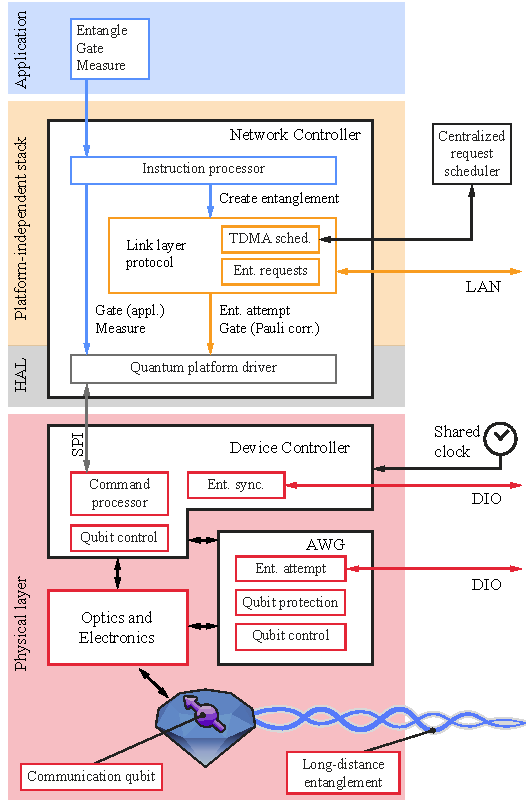
\includegraphics[width=0.6\linewidth]{figures/netnode.pdf}
    \caption{
        Quantum network node architecture. From top to bottom: At the application layer, a simple
        platform-independent routine is sent to the network controller. The network controller
        implements the platform-independent stack --- in this work only the link layer protocol ---
        and a \acrfull{hal} to interface with the physical layer's device controller. An instruction
        processor dispatches instructions either directly to the physical layer, or to the link
        layer protocol in case a remote entangled state is requested by the application. The link
        layer schedules entanglement requests and synchronizes with the remote node (on a local area
        network) using a \acrfull{tdma} schedule computed by a centralized scheduler (external). At
        the physical layer, the device controller fetches commands from --- and replies with
        outcomes to --- the network controller. Driven by a clock shared with the neighboring node,
        it performs hard-real-time synchronization for entanglement generation using a \acrfull{dio}
        interface. By controlling the optical and electronic components (among which an
        \acrlong{awg}, \acrshort{awg}), the device controller can perform universal quantum control
        of the communication qubit in real-time, as well as attempt long-distance entanglement
        generation with the neighboring node.
    }
    \label{fig:netnode}
\end{figure}

The original design of the \acrshort{qegp} and \acrshort{mhp} protocols, as well as our revision,
specifies the conceptual interaction between the two protocols and the service exposed to a higher
layer in the system, but does not impose particular constraints on how to implement link layer and
physical layer, how to realize the physical interface between them, and how to configure things such
as the centralized request scheduler and the entanglement attempt procedure. \Cref{fig:netnode}
gives an overview of the architecture of our quantum network nodes. We briefly describe our most
relevant implementation choices here and in the physical layer section.

\paragraph{Application processing}

At the application layer, user programs --- written in Python using a dedicated \emph{software
development kit}~\cite{netqasm_sdk} --- are processed by a rudimentary compilation stage, which
translates abstract quantum networking applications into gates and operations supported by our
specific quantum physical platform. Such gates and operations are expressed in a low-level
assembly-like language for quantum networking applications called
\emph{NetQASM}~\cite{dahlberg_2022_netqasm}. As part of our software stack, we also include an
\emph{instruction processor}, conceptually placed above the link layer, which is in charge of
dispatching entanglement requests to \acrshort{qegp} and other application instructions to the
physical layer directly.

\paragraph{Interface}

Ref.~\cite{dahlberg_2019_egp} did not provide a specification of the interface to be exposed by the
physical layer. We designed this interface such that the physical layer can accept \emph{commands}
from the higher layer, specifically:
%
\begin{inlinelist}
    \item qubit initialization (\texttt{INI}),
    \item qubit measurement (\texttt{MSR}),
    \item single-qubit gate (\texttt{SQG}),
    \item entanglement attempt (\texttt{ENT}, or \texttt{ENM} for \emph{M}- or \emph{R}-type
          requests),
    \item pre-measurement gates selection (\texttt{PMG}, to specify in which basis to measure the
          qubit for \emph{M}- or \emph{R}-type requests).
\end{inlinelist}
For each command, the physical layer reports back an \emph{outcome}, which indicates whether the
command was executed correctly, and can bear the result of a qubit measurement and the Bell state
produced after a successful entanglement attempt. Our software stack also comprises a
\emph{\acrlong{hal}} (\acrshort{hal}) that sits below \acrshort{qegp} and the instruction processor.
The \acrshort{hal} encodes and serializes commands and outcomes, and is thus used to interface with
the device controller.

\paragraph{\acrshort{tdma} network schedule}

Designing a full-blown centralized request scheduler is a challenge in and of its own, outside the
scope of this work. Instead of implementing such a scheduler, we compute static \acrshort{tdma}
network schedules~\cite{skrzypczyk_2021_arch} and install them manually on the two network nodes
upon initialization. \acrshort{tdma} schedules for our simple single-link experiments are quite
trivial (see Supplementary Material ??), as the network resources of a node are not contended by
multiple links.

\paragraph{Entanglement attempts}

Producing entanglement on a link can take several attempts. To minimize the number of \texttt{ENT}
commands fetched by \acrshort{mhp} from \acrshort{qegp}, as well as to mitigate the \acrshort{mhp}
synchronization overhead incurred after each entanglement command, we batch entanglement attempts at
the \acrshort{mhp} layer, such that synchronization and outcome reporting only happens once per
batch of attempts.

\paragraph{Delivered entangled states}

In our first iteration, we implemented \acrshort{qegp} such that it always delivers $\ket{\Phi^+}$
Bell states to the higher layer. This means that, when the physical layer produces a different Bell
state, \acrshort{qegp} (on the node where the entanglement request originates) issues a single-qubit
gate --- a Pauli correction --- to transform the entangled pair into the $\ket{\Phi^+}$ state (we
abbreviate the four two-qubit maximally entangled Bell states as $\ket{\Phi^\pm} = (\ket{00} \pm
\ket{11})/\sqrt{2}$ and $\ket{\Psi^\pm} = (\ket{01} \pm \ket{10})/\sqrt{2}$). A future version of
\acrshort{qegp} could allow the user to request any Bell state, and could extract the Pauli
correction from \acrshort{qegp} so that the application itself can decide, depending on the use
case, whether to apply the correction or not.

\paragraph{Mismatch verification}

As per our design specification, \acrshort{mhp} should also be responsible for verifying that the
entanglement commands coming from the two \acrshort{qegp} peers belong to the same request. We did
not implement this feature yet because, in our simple quantum network, we do not expect losses on
the classical channel used by the two \acrshort{mhp} parties to communicate --- a lossy classical
channel would be the primary source of inconsistencies at the \acrshort{mhp}
layer~\cite{dahlberg_2019_egp}. However, we believe that this verification step will prove very
useful in real-world networks where classical channels do not behave as predictably.

\paragraph{Deployment}

We implemented \acrshort{qegp} as a software module in a system that also includes the instruction
processor and the hardware abstraction layer. \acrshort{qegp}, the instruction processor and the
hardware abstraction layer, forming the \emph{network controller}, are implemented as a C/C++
standalone runtime developed on top of FreeRTOS, a real-time operating system for embedded
platforms~\cite{freertos}. The runtime and the underlying operating system are deployed on a
dedicated Avnet MicroZed --- an off-the-shelf platform based on the Zynq-7000 SoC, which hosts two
ARM Cortex-A9 processing cores, of which only one is used, clocked at \qty{667}{\MHz}.
\acrshort{qegp} connects to its remote peer via \acrshort{tcp} over a Gigabit Ethernet interface.
The interface to the physical layer is realized through a \qty{12.5}{\MHz} \acrshort{spi}
connection. The user application is sent from a general-purpose 4-core desktop machine running
Linux, which connects to the instruction processor through the same Gigabit Ethernet interface that
\acrshort{qegp} uses to communicate with its peer.

\section{Physical Layer Control in Real-Time}
\label{sec:netstack:phys}

In this section, we outline the design and operation of the physical layer, which executes the
commands issued by the higher layers on the quantum hardware and handles time-critical
synchronization between the quantum network nodes. The physical layer of a quantum network, as
opposed to the apparatus of a physics experiment, needs to be able to execute commands coming from
the layer above in real-time. Additionally, when performing the requested operations, it needs to
leave the quantum device in a state that is compatible with future commands (for example, as
discussed below, it should protect qubits from decoherence while it awaits further instructions).
Finally, if a request cannot be met (e.g.~the local quantum hardware is not ready, the remote
quantum hardware is not available, etc.), the physical layer should notify the link layer of the
issue without interrupting its service.

Our quantum network is composed of two independent nodes based on diamond \acrshort{nv} centers
physically separated by \qty{\approx 2}{m} (see \cref{fig:netnode} for the architecture of one node,
and Supplementary Material ?? for details on the connections between the two nodes). We will refer
to the two nodes as \emph{client} and \emph{server}, noting that this is only a logical separation
useful to describe the case studies --- the two nodes have the exact same capabilities. On each
node, we implement the logic of the physical layer in a state-machine-based algorithm deployed on a
time-deterministic microcontroller, the \emph{device controller} (J\"ager ADwin Pro II, based on
Zynq-7000 SoC, dual-core ARM Cortex-A9, clocked at \qty{1}{\GHz}). Additionally, each node uses an
arbitrary waveform generator (\acrshort{awg}, Zurich Instruments HDAWG8, \qty{2.4}{GSa/s},
\qty{300}{\MHz} sequencer) for nanosecond-resolution tasks, such as fast optical and electrical
pulses; the use of such a user-programmable \acrshort{fpga}-based \acrshort{awg}, as opposed to a
more traditional upload-and-play instrument (such as the ones used in
Ref.~\cite{pompili_2021_multinode}), enables the real-time control of our quantum device.

\paragraph{Single node operation}

On our quantum platform, before a node is available to execute commands, it needs to perform a qubit
readiness procedure called \emph{\acrlong{crcheck}} (\acrshort{crcheck}). This ensures that the
qubit system is in the correct charge state and that the necessary lasers are resonant with their
respective optical transitions. Other quantum platforms might have a similar preparation step, such
as loading and cooling for atoms and ions~\cite{stephenson_2020_highrate, ritter_2012_elementary}.
Once the \acrshort{crcheck} is successful, the device controller can fetch a command from the
network controller. Depending on the nature of the command, the device controller might need to
coordinate with other equipment in the node or synchronize with the device controller of the other
node.

For qubit initialization and measurement commands (\texttt{INI} and \texttt{MSR}), the device
controller shines the appropriate laser for a pre-defined duration
(\texttt{INI}\qty{\approx100}{\us}, \texttt{MSR}\qty{\approx10}{\us}). Both operations are
deterministic and carried out entirely by the device controller.

Single qubit gates (\texttt{SQG}) require the coordination of the device controller and the
\acrshort{awg}. For our communication qubits, they consist of generating an electrical pulse with
the \acrshort{awg} (duration \qty{\approx100}{\ns}), which is then multiplied to the qubit frequency
(\qty{\approx2}{\GHz}), amplified and finally delivered to the quantum device. The link layer can
request rotations in steps of $\pi/16$ around the X, Y or Z axis of the Bloch sphere (here we
implement only X and Y rotations, Z rotations will be implemented in the near future, see
Supplementary Material ??). When a new gate is requested by the link layer, the device controller at
the physical layer informs the \acrshort{awg} of the gate request via a parallel \num{32}-bit
\acrshort{dio} interface. The \acrshort{awg} will then select one of the $64$ pre-compiled
waveforms, play it, and notify the device controller that the gate has been executed. The device
controller will in turn notify the network controller of the successful operation.

After the rotation has been performed, our qubit --- if left idling --- would lose coherence in
\qty{\approx5}{\us}. A coherence time exceeding \qty{1}{s} has been reported on our
platform~\cite{abobeih_2018_one_sec} using decoupling sequences (periodic rotations of the qubit
that shield it from environmental noise). By interleaving decoupling sequences and gates, one can
perform extended quantum computations~\cite{bradley_2019_one_min}. These long sequences of pulses
have in the past been calculated and optimized offline (on a PC), then uploaded to an
\acrshort{awg}, and finally executed on the quantum devices with minimal interaction capabilities
(mostly binary branching trees, see~\cite{pompili_2021_multinode}). In our case, it is impossible to
pre-calculate these sequences, since we cannot know in advance which gates are going to be requested
by the link layer. To solve this challenge, we implement a {qubit protection} module on the
\acrshort{awg}, that interleaves decoupling sequences with the requested gates in real-time. As soon
as the first gate in a sequence is requested, the \acrshort{awg} starts a decoupling sequence on the
qubit. Then, it periodically checks if a new gate has been requested, and if so, it plays it at the
right time in the decoupling sequence. The \acrshort{awg} will continue the qubit protection routine
until the device controller will ask for it to stop (e.g.~to perform a measurement). This technique
allows us to execute universal qubit control without prior knowledge of the sequence to be played,
and --- crucially --- in real-time.

\paragraph{Entanglement generation}

Differently from the commands previously discussed, attempting entanglement generation
(\texttt{ENT}) requires tight timing synchronization between the device controllers --- and
\acrshortpl{awg} --- of the two nodes. In our implementation, the two device controllers share a
common \qty{1}{MHz} clock as well as a \acrshort{dio} connection to exchange synchronization
messages (see Ref.~\cite{pompili_2021_multinode}). When the device controllers are booted, they
synchronize an internal cycle counter that is used for time-keeping, and is shared, at each node,
with their respective network controllers to provide timing information to the link layer and the
higher layers. Over larger distances, one could use well-established protocols to achieve
sub-nanosecond, synchronized, \acrshort{gps}-disciplined common clocks~\cite{whiterabbit}.

When a device controller fetches an \texttt{ENT} command, it starts a three-way handshake procedure
with the device controller of the other node. If the other node has also fetched an \texttt{ENT}
command, they will synchronize and proceed with the entanglement generation procedure. If one of the
two nodes is not available (e.g.~it is still trying to pass the \acrshort{crcheck}) the other node
will time out, after \qty{0.5}{\ms}, and return an \emph{entanglement synchronization failure}
(\texttt{ENT\_SYNC\_FAIL}) to its link layer. The duration of the timeout is chosen such that is
comparable with the average time taken by a node to pass the \acrlong{crcheck} (if correctly on
resonance). This is to avoid unnecessary interactions between physical layer and link layer. After
the entanglement synchronization step, the device controllers proceed with an optical phase
stabilization cycle~\cite{pompili_2021_multinode}, and then the \acrshortpl{awg} are triggered to
attempt entanglement generation. In our implementation, one device controller (the server's)
triggers both \acrshortpl{awg} to achieve sub-nanosecond jitter between the two \acrshortpl{awg}
(see Supplementary Material ?? for a discussion on longer distance implementation). Each
entanglement attempt lasts \qty{3.8}{\us}, and includes fast qubit initialization,
communication-qubit to flying-qubit entanglement, and probabilistic entanglement swapping of the
flying qubits~\cite{pompili_2021_multinode}. The \acrshortpl{awg} attempt entanglement up to
\num{1000} times before timing out and reporting an {entanglement failure} (\texttt{ENT\_FAIL}).
Longer batches of entanglement attempts would increase the probability that one of the nodes goes
into the unwanted charge state (and therefore cannot produce entanglement, see Supplementary
Material ??). While in principle possible, we did not implement, in this first realization, the
charge stabilization mechanism proposed in Ref.~\cite{humphreys_2018_delivery} that would allow for
significantly longer batches of entanglement attempts.

If an entanglement generation attempt is successful (probability \num{\approx 5e-5}), the
communication qubits of the two nodes will be projected into an entangled state (either
$\ket{\Psi^+}$ or $\ket{\Psi^-}$, depending on which detector clicked at the heralding station). To
herald success of the entanglement attempt, a \acrshort{cpld} (\acrlong{cpld}, Altera MAX V
5M570ZF256C5N) sends a fast digital signal to both \acrshortpl{awg} and device controllers, to
prevent a new entanglement attempt from being played (which would destroy the generated entangled
state). When the heralding signal is detected, the \acrshortpl{awg} enter the qubit protection
routine and wait for further instructions from the device controllers, which in turn notify the link
layer of the successful entanglement generation, as well as which state was generated.

To satisfy \emph{M}- or \emph{R}-type entanglement requests, the link layer can instruct the
physical layer to apply an immediate measurement to the entangled qubit by means of an \texttt{ENM}
command. Up until heralding of the entangled state, the physical layer operates as it does for the
\texttt{ENT} command. When the state is ready, it proceeds immediately with a sequence of single
qubit gates (as prescribed by an earlier \texttt{PMG} command) and a qubit measurement. The result
of the measurement, together with which entangled state was generated, is communicated to the link
layer. It is worth noting that the two nodes could fetch different types of requests and still
generate entanglement. In fact, this will be used later in the remote state preparation application.

\section{Evaluation}
\label{sec:netstack:eval}

\begin{figure}
    \centering
    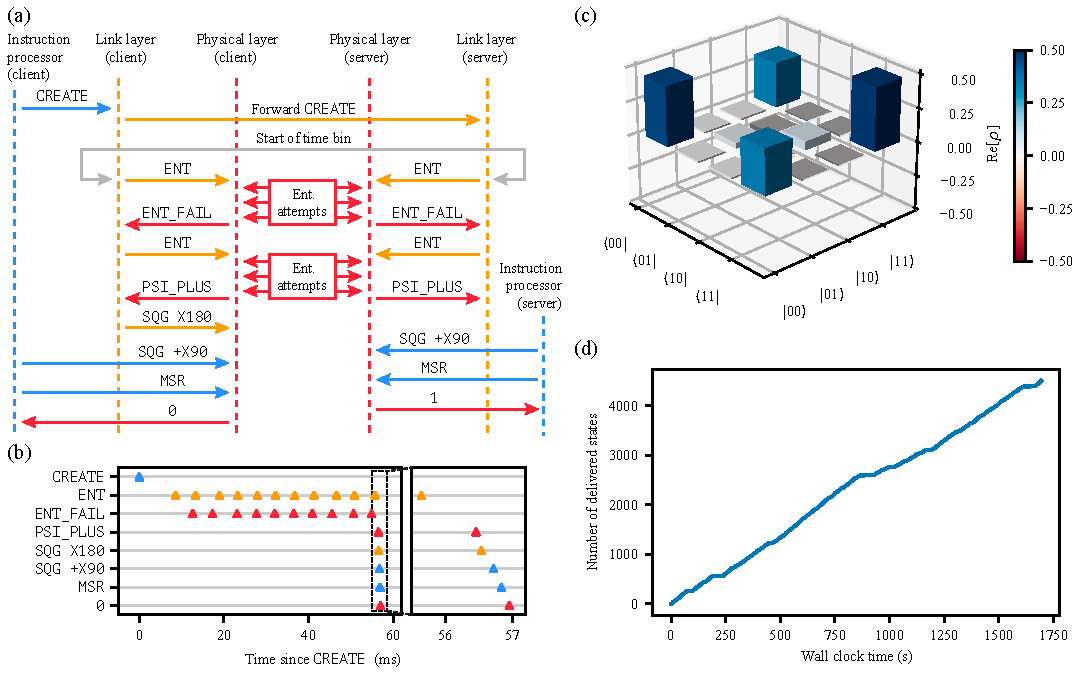
\includegraphics[width=\linewidth]{figures/fstomography.pdf}
    \caption{
        Full state tomography with the quantum network stack.
        %
        (a) Sequence diagram of the communication steps across the network stack and the two nodes
        to perform one repetition of the tomography application (in particular, measurement of the
        $\braket{YY}$ correlator). The coloring follows that of \cref{fig:netstack}.
        \texttt{CREATE}: entanglement request, \texttt{ENT}: entanglement attempts request,
        \texttt{ENT\_FAIL}: failed the batch of entanglement attempts, \texttt{PSI\_PLUS}:
        successful entanglement attempt with generated state $\Psi^+$, \texttt{SQG}: single-qubit
        gate, \texttt{X180}: \ang{180} rotation around X axis, \texttt{MSR}: qubit measurement,
        \texttt{0/1}: qubit measurement outcome. See \cref{tab:link_possible_outcomes} for a
        complete list of commands. Note that the client's link layer protocol requests a
        \texttt{X180} gate after entanglement generation to deliver the $\ket{\Phi^+}$ Bell state to
        the higher layer.
        %
        (b) Example time trace of (a) for the client. Several batches of entanglement attempts are
        required before an entangled state is heralded. On the right, a zoomed-in part of the trace
        (corresponding to the dashed box in the left plot).
        %
        (c) Reconstructed density matrix of the states delivered by the link layer. Only the real
        part is plotted (imaginary elements are all \num{\approx 0}, see main text). We estimate a
        fidelity F with $\ket{\Phi^+}$ of $F =$ \num{0.783(7)}.
        %
        (d) Total number of delivered states over time. The occasional pauses in entanglement
        delivery (plateaus) are due to the client's \acrshort{nv} center becoming off-resonant with
        the relevant lasers (see \cref{sec:link_suppl_off_resonant}). Differences in slope are due
        to changes in resonance conditions that increase the time necessary to pass the
        \acrlong{crcheck}.
    }
    \label{fig:fstomography}
\end{figure}

To demonstrate and benchmark the capabilities of the link layer protocol, the physical layer, and of
our system as a whole, we execute --- on our two-node network --- three quantum networking
applications, all having a similar structure: the client asks for an entangled pair with the server,
which \acrshort{qegp} delivers in the $\ket{\Phi^+}$ Bell state, and then both client and server
measure their end of the pair in a certain basis. First, we perform full quantum state tomography of
the delivered entangled states. Second, we request and characterize entangled states of varying
fidelity. Third, we execute remote preparation of qubit states on the server by the client. For all
three applications, we study the quality of the entangled pairs delivered by our system.
Additionally, we use the second application to assess the latency incurred by our link layer, and to
compare it to the overall entanglement generation latency, including that of the physical layer.
Crucially, the three applications are executed back-to-back on the quantum network, without any
software or hardware changes to the system --- the only difference being the
quantum-platform-independent application sent to the instruction processor (see Supplementary
Material ??).

The sequence diagram in \cref{fig:fstomography}a exemplifies the general flow between system
components during the execution of an application. At first, the instruction processor issues a
request to create entanglement to link layer (\texttt{CREATE}). Then, the client's link layer
forwards the request with the server's counterpart (Forward \texttt{CREATE}). The request is
processed as soon as the designated time bin in the \acrshort{tdma} schedule starts, at which point
the first entanglement command (\texttt{ENT}) is fetched by physical layer. After an entangled state
is produced successfully (\texttt{PSI\_PLUS}), the link layer of the client issues, if needed, a
Pauli correction ($\pi$ rotation around the X axis, \texttt{SQG X180}) to deliver the pair in the
$\ket{\Phi^+}$ state. Finally, the instruction processor issues a gate ($\pi/2$ rotation around the
X axis, \texttt{SQG X90}) and a measurement (\texttt{MSR}) to read out the entangled qubit in a
certain basis, and receives an outcome from the physical layer (\texttt{0}).
\Cref{fig:fstomography}b illustrates the actual latencies between these interactions in one
iteration of the full state tomography application.

For all our experiments, we configured \acrshort{tdma} time bins to be of \qty{20}{\ms}. In a larger
network, the duration of time bins should be calibrated according to the average time it takes, on a
certain link, to produce an entangled pair of a certain fidelity~\cite{skrzypczyk_2021_arch}. By
doing so, one can maximize network usage and thus reduce qubit decoherence on longer end-to-end
paths. However, in our single-link network, the duration of time bins only influences the frequency
at which new entanglement requests are processed. Our time bin duration accommodates up to four
batches of \num{1000} entanglement attempts.

\paragraph{Full quantum state tomography}

The first application consists in generating entangled states at the highest \emph{minimum fidelity}
currently available on our physical setup (\num{0.80}), and measuring the two entangled qubits in
varying bases to learn their joint quantum state. We measure all \num{9} two-node correlators
($\braket{\mathrm{XX}}, \braket{\mathrm{XY}}$, ...,~$\braket{\mathrm{ZZ}}$) as well as all their
$\pm$ variations ($\braket{\mathrm{+X+X}}, \braket{\mathrm{+X-X}}$, etc.) to minimize the bias due
to measurement errors. For each of the $9 \times 4 = 36$ combinations, we measure \num{125} data
points, for a total of \num{4500} entangled states generated and measured. The Supplementary
Material ?? contains a pseudocode description of the application.

The collected measurement outcomes are then analyzed using QInfer~\cite{granade_2017_qinfer}, in
particular the Monte Carlo method described in Ref.~\cite{granade_2016_practical} for Bayesian
estimation of density matrices from tomographic measurements. The reconstructed density matrix is
displayed in \cref{fig:fstomography}c (only the real part is shown in the figure) and its values and
uncertainties are
%
\begin{equation*}
    \mathrm{Re}[\rho] = \begin{pmatrix}
        0.442(6) & 0.003(3)  & 0.003(2)  & 0.328(5)  \\
        0.003(3) & 0.033(6)  & -0.023(5) & -0.000(5) \\
        0.003(2) & -0.023(5) & 0.056(4)  & -0.003(4) \\
        0.328(5) & -0.000(5) & -0.003(4) & 0.469(7)  \\
    \end{pmatrix},
\end{equation*}
%
\begin{equation*}
    \mathrm{Im}[\rho] = \begin{pmatrix}
        0         & -0.014(3) & -0.005(7) & 0.032(5)  \\
        0.014(3)  & 0         & -0.002(4) & 0.001(5)  \\
        0.005(7)  & 0.002(4)  & 0         & -0.000(7) \\
        -0.032(5) & -0.001(5) & 0.000(7)  & 0         \\
    \end{pmatrix}.
\end{equation*}
Here $\rho_{ij, mn} = \braket{ij|\ \rho\ |mn}$, with $i,m$ ($j,n$) being the client (server) qubit
states in the computational basis. The uncertainty on each element of the density matrix is
calculated as the standard deviation of that element over the probability distribution approximated
by the Monte Carlo reconstruction algorithm (probability distribution approximated by \num{1E5}
Monte Carlo particles~\cite{granade_2016_practical}). It is then possible to estimate the fidelity
of the delivered entangled states with respect to the maximally entangled Bell state, which we find
to be $F =$ \num{0.783(7)}. The measured fidelity is slightly lower (\qty{\approx 3}{\percent}) than
what measured in Ref.~\cite{pompili_2021_multinode} without the use of the \acrshort{qegp}
abstraction (and the whole network controller where \acrshort{qegp} runs). This discrepancy could be
due to the additional physical-layer decoupling sequences required for real-time operation
(\qty{\approx 300}{\us}) and the additional single-qubit gate issued by the link layer to always
deliver $\ket{\Phi^+}$ (see Supplementary Material ??).

It is to be noted that, in order to obtain the most faithful estimate of the generated state (see
Supplementary Material ?? for details), the measured expectation values are corrected, in
post-processing, to remove known tomography errors of both client and
server~\cite{nachman_2020_unfolding}, and events in which at least one physical device was in the
incorrect charge state.

Finally, we show, in \cref{fig:fstomography}d, that our system can sustain a fairly stable
entanglement delivery rate over \qty{\approx 30}{min} of data acquisition --- plateaus and changes
in slope can be attributed to varying conditions of resonance between the \acrshort{nv} centers and
the relevant lasers (see Supplementary Material ??).

\paragraph{Latency vs fidelity}

The \acrshort{qegp} interface allows its user to request entangled pairs at various minimum
fidelities. For physical reasons, higher fidelities will result in lower entanglement generation
rates~\cite{stockill_2017_phasetuned, humphreys_2018_delivery}. The trade-off between fidelity and
throughput is particularly interesting in a scenario where some applications might require
high-fidelity entangled pairs and are willing to wait a longer time, while others might prefer
lower-fidelity states but higher rates~\cite{dahlberg_2019_egp}. Clearly, for the link layer to
offer a range of fidelities to choose from, the underlying physical layer must support such a range.
We benchmark the capabilities of the link layer and of the physical layer to deliver states at
various fidelities in a single application by measuring the $\braket{\mathrm{XX}}$,
$\braket{\mathrm{YY}}$ and $\braket{\mathrm{ZZ}}$ correlators (and their $\pm$ variations, as we did
above, for a total of $3 \times 4 = 12$ correlators) for seven different target fidelities,
(\num{0.50}, \num{0.55}, \num{0.60}, \num{0.65}, \num{0.70}, \num{0.75}, \num{0.80}). We generate
\num{1500} entangled states per fidelity, for a total of \num{10500} delivered states (see
Supplementary Material ??). With this case study, we analyze both the resulting fidelity and the
system's latency for different requested fidelities.

\begin{figure}
    \centering
    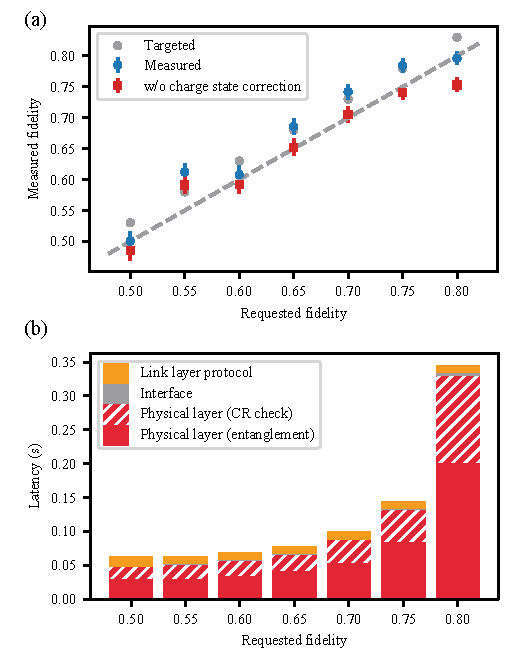
\includegraphics[width=0.6\linewidth]{figures/latencyvsfid.pdf}
    \caption{
        Performance of the entanglement delivery service.
        %
        (a) Measured fidelity of the states delivered by the link layer for varying requested
        fidelity. Targeted fidelity at the physical layer is 0.03 higher than the link layer
        protocol's \emph{minimum fidelity} request. When not correcting for wrong charge state
        events, fidelity is reduced by a few percents (see \cref{sec:link_suppl_m_corr}). Error bars
        represent \num{1} s.d.
        %
        (b) Average latency of the entanglement delivery per requested fidelity, broken down into
        sources of latency. Entanglement generation and \acrlong{crcheck} at the physical layer are
        the largest sources of latency (at higher fidelities, more entanglement attempts are
        required before success). Running the link layer protocol introduces a small but measurable
        overhead (\qty{\approx 10}{ms}) to the entanglement generation procedure, which does not
        depend on the requested fidelity, and that could be mitigated by requesting multiple
        entangled states in a single instruction. The communication delays between quantum network
        controller and quantum device controller (Interface) introduce negligible overall latency.
    }
    \label{fig:latencyvsfid}
\end{figure}

The results for measured fidelity versus requested fidelity are shown in \cref{fig:latencyvsfid}a.
It is worth noting that the application iterates over the range of fidelities in real-time, and thus
the physical layer is prepared to deliver any of them at any point. We calibrate the physical layer
to deliver states of slightly higher fidelity than the requested ones (\num{0.03} more), since
entanglement requests specify the \emph{minimum} desired fidelity. The measured fidelities are ---
within measurement uncertainty --- always matching or exceeding the requested minimum ones (the
dashed gray line in \cref{fig:latencyvsfid}a is the $y=x$ diagonal). As in the previous application,
measurement outcomes are post-processed to eliminate tomography errors and events in which the
physical devices were in the incorrect charge state (we refer to the latter as \emph{charge state
correction}). For arbitrary applications that use the delivered entangled states for something other
than statistical measurements, applying the second correction directly at the link layer might prove
challenging, since the information concerning whether to discard an entangled pair is only available
at the physical layer \emph{after} the entangled state is delivered to the link layer (when the next
\acrshort{crcheck} is performed). However, a mechanism to identify \emph{bad} entangled pairs
retroactively at the link layer --- like the expiry functionality included in the original design of
\acrshort{qegp}~\cite{dahlberg_2019_egp} --- could be used to discard entangled states after they
have been delivered by the physical layer. For completeness, we also report, again in
\cref{fig:latencyvsfid}a, the measured fidelity when the wrong charge state correction is not
applied.

For each requested fidelity we also measure the entanglement generation
latency~\cite{dahlberg_2019_egp}, defined as the time between the issuing of the \texttt{CREATE}
request to the link layer, until the successful entanglement outcome reported by the physical layer
(refer to \cref{fig:fstomography}a for a diagram of the events in between these two).
\Cref{fig:latencyvsfid}b shows the measured average latency, grouped by requested fidelity and
broken down into the various sources of latency. When calculating the average latencies, we have
ignored entanglement requests that required more than \qty{10}{s} to be fulfilled. These
high-latency requests correspond to the horizontal plateaus of \cref{fig:fstomography}d (see
Supplementary Material ?? for details). The main contribution to the total latency comes from the
entanglement generation process at the physical layer, followed by the \acrshort{nv} center
preparation time (\acrshort{crcheck}). Both latency values are consistent with the expected number
of entanglement attempts required by the single-photon entanglement protocol employed at the
physical layer~\cite{humphreys_2018_delivery}. The link layer protocol adds, on average,
\qty{\approx 10}{\ms} of extra latency to all requests, regardless of their fidelity. This is due
partly to the synchronization of the \texttt{CREATE} request between the two nodes (i.e.~a simple
\acrshort{tcp} message), but mostly to the nodes having to wait for the next time bin in the network
schedule to start (the larger the time bins, the larger the worst-case waiting time, see
Supplementary Material ??). We remark that, by requesting multiple entangled states in a single
\texttt{CREATE}, one can distribute this overhead over many generated pairs, to the point where it
becomes negligible. While our applications did not issue multi-pair \texttt{CREATE} requests, this
would be the more natural choice for real applications, and would result in better utilization of
the allocated time bins. Finally, the overhead incurred by the interface between microcontrollers is
rather small (barely visible in \cref{fig:latencyvsfid}b), but could however be further reduced by
integrating device controller and network controller into a single device. It is worth mentioning
that, in our simple scenario in which each entanglement request is only submitted to \acrshort{qegp}
after the previous one completes, and thus the request queue never grows larger than one element,
throughput happens to be almost exactly the same as the inverse of latency, and hence it is not
reported here.

Overall, we observe that the extra entanglement generation latency incurred when deploying an
abstraction layer (\acrshort{qegp}) on top of the physical layer, while not too modest, is only a
small part of the whole, particularly at higher fidelities. Nevertheless, optimizing the length of
\acrshort{tdma} time bins could result in an even smaller overhead (see Supplementary Material ??).

\begin{figure}
    \centering
    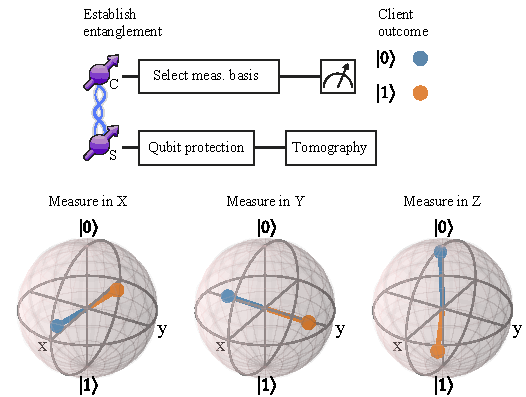
\includegraphics[width=0.6\linewidth]{figures/rsprep.pdf}
    \caption{
        Tomography of states prepared on the server by the remote client. For each chosen
        measurement axis of the client (X, Y, Z), and for each obtained measurement outcome at the
        client ($\ket{0}$, $\ket{1}$), a different state is prepared on the server. Plotted on the
        Bloch spheres are the results of the tomography on the server's qubit. Uncertainties on each
        coordinate are \num{\approx 0.05} (see \cref{sec:link_suppl_m_corr}). We find an average
        preparation fidelity of $F =$ \num{0.853(8)}.
    }
    \label{fig:rsprep}
\end{figure}

\paragraph{Remote state preparation}

One of the use cases of the \acrshort{qegp} service is to prepare quantum states on a remote quantum
server~\cite{dahlberg_2019_egp}. Remote state preparation is a fundamental step to execute a blind
quantum computation application~\cite{broadbent_2009_ubqc}, whereby a client quantum computer with
limited resources can run quantum applications on a powerful remote quantum server using the many
qubits the server has, while keeping the performed computation private.

Remote state preparation is different from the previous two cases in that the client can measure its
end of the entangled pair as soon as the pair is generated, while the server has to keep its qubit
alive waiting for further instructions. For such a scenario, the client can make use of
\acrshort{qegp}'s service to issue \emph{R}-type entanglement requests, so that the local end of the
entangled pair can be measured (in a certain basis) as soon as it is generated, while the server's
qubit can be protected for later usage. An \emph{R}-type entanglement request results in an
\texttt{ENM} command on the client and an \texttt{ENT} command on the server. For this type of
requests (as well as for \emph{M}-type ones), since the local end of the pair is measured
immediately, the client's \acrshort{qegp} can skip the Pauli correction used to always deliver
$\ket{\Phi^+}$, and can instead apply a classical correction to the received measurement outcome
(see Supplementary Material ??).

To showcase this feature of \acrshort{qegp} we use the client node to prepare the six cardinal
states on the server ($\ket{\pm x}$, $\ket{\pm y}$, $\ket{0}$ and $\ket{1}$) by having the client
measure its share of the entangled state in the six cardinal bases. We then let the server measure
the prepared states --- again in the six cardinal bases --- to perform tomography. For each client
measurement basis, and for each server tomography basis, we deliver \num{125} entangled states at a
requested fidelity of \num{0.80}, for a total of $6 \times 6 \times 125 = 4500$ remote state
preparations (see Supplementary Material ??). The results are presented in \cref{fig:rsprep}, which
displays the tomography of the prepared states on the server, for the three different measurement
axes of the client and the two possible measurement outcomes of the client. The prepared states are
affected by the measurement error of the client ($F_0 =$ \num{0.928(3)}, $F_1 = $ \num{0.997(1)}):
an error in the measurement of the client's qubit results in an incorrect identification of the
state prepared on the server. By alternating between positive and negative readout orientations, we
make sure that the errors affect all prepared states equally, instead of biasing the result. We note
that we exclude, once again, events in which at least one of the two devices was in the wrong charge
state, and we correct for the known tomography error on the server (results without corrections are
in the Supplementary Material ??). Overall, we find an average remote state preparation fidelity of
$F =$ \num{0.853(8)}. The asymmetry in the fidelity of the $\ket{0}$ and $\ket{1}$ states is caused
by the asymmetry in the populations $\braket{01|\ \rho\ |01}$ vs $\braket{10|\ \rho\ |10}$ of the
delivered entangled state, which in turn is due to the double $\ket{0}$ occupancy error of the
single-photon protocol used to generate entanglement~\cite{humphreys_2018_delivery,
pompili_2021_multinode}.

\section{Discussion}

In summary, we have demonstrated the operation of a link layer and a physical layer for
entanglement-based quantum networks. The link layer abstracts the entanglement generation procedure
provided by the physical layer --- implemented here with two \acrshort{nv} center-based quantum
network nodes --- into a robust platform-independent service that can be used to run quantum
networking applications. We performed full quantum state tomography of the states delivered by the
link layer, tested its ability to deliver states at different fidelities in real-time, and verified
remote state preparation of a qubit from the client on the server, a fundamental step towards blind
quantum computation~\cite{broadbent_2009_ubqc}. We have shown that our implementation of link and
physical layers can deliver entangled states at the fidelity requested by the user, despite some
marginal inefficiencies --- some of which can be addressed in a future version of the protocols
(e.g.~avoiding Pauli corrections unless necessary). We have also quantified the additional latency
incurred by deploying the link layer protocol on top of the physical layer. Although not
detrimental, the extra overhead is still noticeable, but can also be scaled down by optimizing the
scheduling of entanglement generation requests. We also acknowledge that scheduling a quantum node's
resources is still an open problem~\cite{skrzypczyk_2021_arch, vardoyan_2019_performance,
vardoyan_2021_capacity} and that the simple approach taken here is likely a suboptimal choice for
more advanced quantum networks. We emphasize, however, that our link layer protocol is not tied to
any particular scheduling algorithm or architecture --- it merely expects that the schedule of each
node be matched with its peer. In Ref.~\cite{dahlberg_2019_egp} for example, the schedule was
instead formed via a distributed queue protocol, and in the future other architectures and
algorithms~\cite{skrzypczyk_2021_arch} may be more suitable for scaling to larger networks.

Other research challenges posed by our work include an in-depth analysis of the security of quantum
network implementations. For example, it is clear that if the classical control messages used in our
protocol are not authenticated, unwanted entanglement generation may be triggered at one of the
nodes. In some physical layer implementations such as the one considered here, this may negatively
impact the quality of the qubits already stored at the node~\cite{kalb_2018_dephasing}, and hence
impact availability. Initial work indicates that the performance impact of adding authentication,
however, is small (refer to \cref{chp:doa}).

The adoption of the techniques presented here (which are not specific to our diamond devices) by
other quantum network platforms~\cite{ritter_2012_elementary, stockill_2017_phasetuned,
rose_2018_observation, nguyen_2019_quantum, stephenson_2020_highrate, trusheim_2020_transform,
son_2020_developing} will boost the development towards large-scale and heterogeneous quantum
networks. Real-time control of memory qubits, as well as the availability of multi-node networks and
dynamic network schedules, will enable demonstrations of the higher layers of the network
stack~\cite{kozlowski_2019_towards}, which in turn will open the door to end-to-end connectivity on
a platform-independent quantum network.

\printbibliography[heading=subbibintoc,title={References}]
